\documentclass[]{article}
\usepackage{lmodern}
\usepackage{amssymb,amsmath}
\usepackage{ifxetex,ifluatex}
\usepackage{fixltx2e} % provides \textsubscript
\ifnum 0\ifxetex 1\fi\ifluatex 1\fi=0 % if pdftex
  \usepackage[T1]{fontenc}
  \usepackage[utf8]{inputenc}
\else % if luatex or xelatex
  \ifxetex
    \usepackage{mathspec}
  \else
    \usepackage{fontspec}
  \fi
  \defaultfontfeatures{Ligatures=TeX,Scale=MatchLowercase}
\fi
% use upquote if available, for straight quotes in verbatim environments
\IfFileExists{upquote.sty}{\usepackage{upquote}}{}
% use microtype if available
\IfFileExists{microtype.sty}{%
\usepackage{microtype}
\UseMicrotypeSet[protrusion]{basicmath} % disable protrusion for tt fonts
}{}
\usepackage[margin=1in]{geometry}
\usepackage{hyperref}
\hypersetup{unicode=true,
            pdftitle={Automate the Browser with Selenium and Python},
            pdfauthor={Davide Lorino},
            pdfborder={0 0 0},
            breaklinks=true}
\urlstyle{same}  % don't use monospace font for urls
\usepackage{graphicx,grffile}
\makeatletter
\def\maxwidth{\ifdim\Gin@nat@width>\linewidth\linewidth\else\Gin@nat@width\fi}
\def\maxheight{\ifdim\Gin@nat@height>\textheight\textheight\else\Gin@nat@height\fi}
\makeatother
% Scale images if necessary, so that they will not overflow the page
% margins by default, and it is still possible to overwrite the defaults
% using explicit options in \includegraphics[width, height, ...]{}
\setkeys{Gin}{width=\maxwidth,height=\maxheight,keepaspectratio}
\IfFileExists{parskip.sty}{%
\usepackage{parskip}
}{% else
\setlength{\parindent}{0pt}
\setlength{\parskip}{6pt plus 2pt minus 1pt}
}
\setlength{\emergencystretch}{3em}  % prevent overfull lines
\providecommand{\tightlist}{%
  \setlength{\itemsep}{0pt}\setlength{\parskip}{0pt}}
\setcounter{secnumdepth}{0}
% Redefines (sub)paragraphs to behave more like sections
\ifx\paragraph\undefined\else
\let\oldparagraph\paragraph
\renewcommand{\paragraph}[1]{\oldparagraph{#1}\mbox{}}
\fi
\ifx\subparagraph\undefined\else
\let\oldsubparagraph\subparagraph
\renewcommand{\subparagraph}[1]{\oldsubparagraph{#1}\mbox{}}
\fi

%%% Use protect on footnotes to avoid problems with footnotes in titles
\let\rmarkdownfootnote\footnote%
\def\footnote{\protect\rmarkdownfootnote}

%%% Change title format to be more compact
\usepackage{titling}

% Create subtitle command for use in maketitle
\newcommand{\subtitle}[1]{
  \posttitle{
    \begin{center}\large#1\end{center}
    }
}

\setlength{\droptitle}{-2em}

  \title{Automate the Browser with Selenium and Python}
    \pretitle{\vspace{\droptitle}\centering\huge}
  \posttitle{\par}
    \author{Davide Lorino}
    \preauthor{\centering\large\emph}
  \postauthor{\par}
      \predate{\centering\large\emph}
  \postdate{\par}
    \date{2018-08-17}


\begin{document}
\maketitle

\begin{figure}
\centering
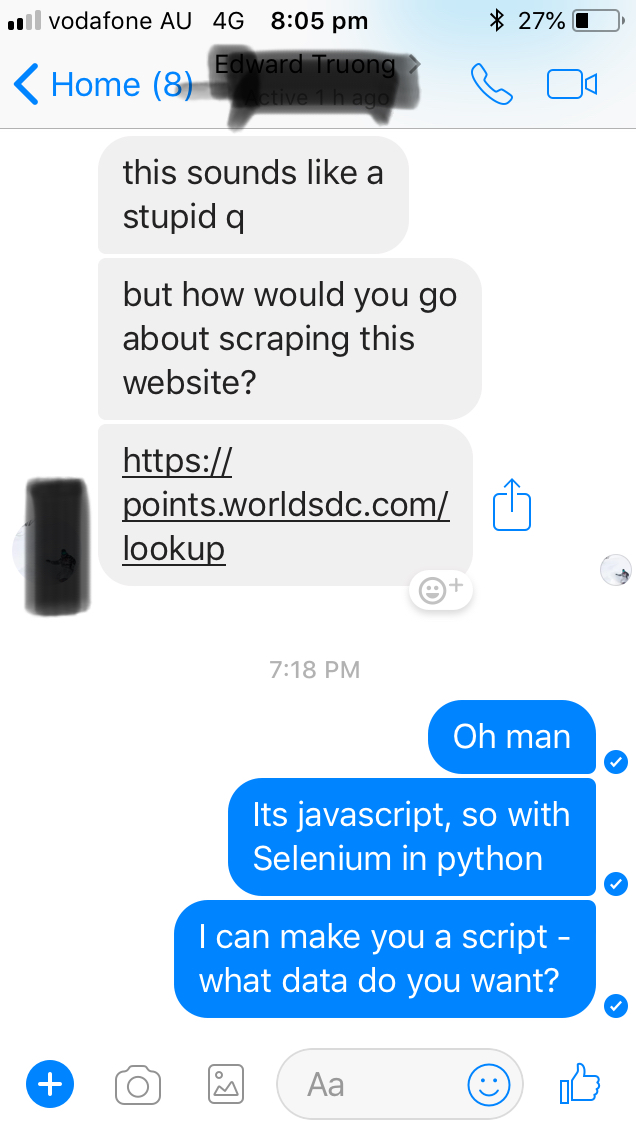
\includegraphics{Scrape.jpeg}
\caption{Scrape}
\end{figure}

\section{Q: How do you scrape data off a website that's rendered in
Javascript?}\label{q-how-do-you-scrape-data-off-a-website-thats-rendered-in-javascript}

\section{A: The Selenium module in
Python.}\label{a-the-selenium-module-in-python.}

In this post I will go over he can use Selenium in Python to interact
with website objects that are rendered in javascript so that we can do
things like:

\begin{itemize}
\tightlist
\item
  Hover-over dropdown menus
\item
  Select sub-menus
\item
  Fill in text entry fields such as username and password to perform
  login operations
\item
  Basically use the .click() and .find\_element\_by\_xpath() functions
  to do everything
\end{itemize}

Building a webscraper/crawler to programmatically pull data from the
internet is a really commonly sought after skill. Most businesspeople
put together reports that are usually some sort of aggregation on
multiple csv files that all need to get pooled together and joined in a
summarized form.

Because of the iterative nature of these reports (daily, weekly,
monthly, quarterly) the process of requesting and pooling the data
together can be extremely tedious, especially if you have lots of data
in different places.

For this, we need the Selenium module in Python. We can pre-generate a
script that will fetch our data each and every time we want to run a
report - the only thing that we will change in our script between
iterations will be the date variables so that we arent just pulling data
for the exact same date or range every time (we will want different data
otherwise theres no point doing more than one of the same report).

\subsubsection{Load the Required Python
Modules}\label{load-the-required-python-modules}

from selenium import webdriver from
selenium.webdriver.common.action\_chains import ActionChains import time

Selenium imports a set of functions that allow us to automate browser
interactions with javascript rendered websites such as ipScape.

Time is a module for declaring when to pause the script and for how long
in order to allow for certain operations to complete before the script
races ahead of where the browser is actually at. The impact of this is
that when the script looks for variables on the page they will not have
been rendered yet and the script will throw an error and not proceed.
For this reason we make use of the function \texttt{time.sleep(3)} where
(3) denotes the number of seconds you want to wait.

\paragraph{Store Username and Password in Python to Pass to the Reports
Login
Page}\label{store-username-and-password-in-python-to-pass-to-the-reports-login-page}

\{python\} usernameStr = `A\_Username' passwordStr = `A\_Password'

\paragraph{Store the Date in Python}\label{store-the-date-in-python}

The dates ``From'' and ``To'' will be sent to the ipScape date filters
for the report that we run. For this reason, we will change the dates in
the below command to suit the date range that we are trying to capture.
Here we have declared August 11th to August 16th, so we will download
data corresponding to this date range when the script runs.

This is the only part of the script that we need to interact with - have
fun!

date\_From = ``11/08/2018 00:00:00'' date\_To = ``16/08/2018 00:00:00''

\paragraph{Load the Required Webdriver - Here we use the Google Chrome
driver}\label{load-the-required-webdriver---here-we-use-the-google-chrome-driver}

browser = webdriver.Chrome(`/Users/Davide/Downloads/chromedriver')

\paragraph{Navigate to the Page}\label{navigate-to-the-page}

browser.get(`\url{https://winepeoplev5.ipscape.com.au/workspace}')

\paragraph{Store an Actions Object from the Selenium Module for
Interacting with Javascript Rendered Page
Objects}\label{store-an-actions-object-from-the-selenium-module-for-interacting-with-javascript-rendered-page-objects}

action = ActionChains(browser)

\paragraph{Find the Username Field in the Login Form and Enter
Username}\label{find-the-username-field-in-the-login-form-and-enter-username}

username = browser.find\_element\_by\_class\_name(`login\_text')

username.send\_keys(usernameStr)

\paragraph{Find the Password Field and Enter
Password}\label{find-the-password-field-and-enter-password}

password = browser.find\_element\_by\_class\_name

password = browser.find\_element\_by\_name(`pwd')

password.send\_keys(passwordStr)

\paragraph{Find and Click Login}\label{find-and-click-login}

login = browser.find\_element\_by\_id(`loginbttn')

login.click()

\paragraph{Go to the First Reports
Page}\label{go-to-the-first-reports-page}

report1 = browser.find\_element\_by\_link\_text(`Live Reports')

report1.click()

\paragraph{Hover Over the Administration
Dropdown}\label{hover-over-the-administration-dropdown}

time.sleep(5)

historical\_reports =
browser.find\_element\_by\_xpath('//*{[}@id="ui-id-10"{]}')

time.sleep(3)

historical\_reports.click()

time.sleep(5)

firstLevelMenu =
browser.find\_element\_by\_xpath('//*{[}@id="header\_container"{]}/nav/div/ul/li{[}2{]}/a')

action.move\_to\_element(firstLevelMenu).perform()

time.sleep(2)

\paragraph{Find and Click the Reports Subheading of the Administration
Dropdown}\label{find-and-click-the-reports-subheading-of-the-administration-dropdown}

secondLevelMenu =
browser.find\_element\_by\_xpath('//*{[}@id="report-management-dialog-invoke"{]}')

action.move\_to\_element(secondLevelMenu).perform()

secondLevelMenu.click()

time.sleep(4)

search\_reports =
browser.find\_element\_by\_xpath('//*{[}@id="report\_search\_string"{]}')

search\_reports.send\_keys(``Historical Inbound Upsell'')

time.sleep(2)

search\_report\_again =
browser.find\_element\_by\_xpath('//*{[}@id="report\_search\_button"{]}')

time.sleep(1)

search\_report\_again.click()

time.sleep(6)

edit\_report\_again =
browser.find\_element\_by\_xpath('//*{[}@id="report-list-table"{]}/tbody/tr/td{[}4{]}/button{[}2{]}/a')

time.sleep(2)

edit\_report\_again.click()

time.sleep(2)

filter\_report\_again =
browser.find\_element\_by\_xpath('//*{[}@id="ui-accordion-report-create-edit-accordion-header-1"{]}')

time.sleep(2)

filter\_report\_again.click()

time.sleep(3)

campaign\_again =
browser.find\_element\_by\_xpath('//*{[}@id="report-filters-table"{]}/tbody/tr{[}1{]}/td{[}2{]}/label/select')

time.sleep(2)

campaign\_again.click()

time.sleep(2)

campaign\_is\_in\_again =
browser.find\_element\_by\_xpath('//*{[}@id="report-filters-table"{]}/tbody/tr{[}1{]}/td{[}2{]}/label/select/option{[}2{]}')

time.sleep(2)

campaign\_is\_in\_again.click()

time.sleep(2)

call\_outcome\_again =
browser.find\_element\_by\_xpath('//*{[}@id="report-filters-table"{]}/tbody/tr{[}2{]}/td{[}2{]}/label/select')

time.sleep(2)

call\_outcome\_again.click()

time.sleep(2)

call\_outcome\_again\_is\_in =
browser.find\_element\_by\_xpath('//*{[}@id="report-filters-table"{]}/tbody/tr{[}2{]}/td{[}2{]}/label/select/option{[}2{]}')

time.sleep(2)

date\_time\_range\_again =
browser.find\_element\_by\_xpath('//*{[}@id="report-filters-table"{]}/tbody/tr{[}3{]}/td{[}2{]}/label/select')

time.sleep(4)

date\_time\_range\_again.click()

date\_time\_range\_again.click()

date\_time\_range\_again.click()

date\_time\_range\_again.click()

time.sleep(4)

date\_time\_range\_again\_is\_range =
browser.find\_element\_by\_xpath('//*{[}@id="report-filters-table"{]}/tbody/tr{[}3{]}/td{[}2{]}/label/select/option{[}3{]}')

time.sleep(4)

date\_time\_range\_again\_is\_range.click()

date\_time\_range\_again\_is\_range.click()

date\_time\_range\_again\_is\_range.click()

date\_time\_range\_again\_is\_range.click()

time.sleep(2)

filter\_bar =
browser.find\_element\_by\_xpath('//*{[}@id="ui-accordion-report-create-edit-accordion-header-1"{]}')

time.sleep(4)

filter\_bar.click()

time.sleep(10)

date\_from\_agen =
browser.find\_element\_by\_name(``filter\_value\_from{[}14010790{]}'')

time.sleep(2)

date\_from\_agen.clear()

date\_from\_agen.send\_keys(date\_From)

time.sleep(3)

date\_to\_agen =
browser.find\_element\_by\_name(``filter\_value\_to{[}14010790{]}'')

time.sleep(2)

date\_to\_agen.clear()

date\_to\_agen.send\_keys(date\_To)

time.sleep(2)

save\_report\_again =
browser.find\_element\_by\_xpath('//*{[}@id="save-report-button"{]}')

time.sleep(2)

save\_report\_again.click()

time.sleep(5)

put\_report\_on\_page\_again =
browser.find\_element\_by\_xpath('//*{[}@id="put-report-button"{]}')

time.sleep(2)

put\_report\_on\_page\_again.click()

time.sleep(3)

expand\_rows\_third\_report =
browser.find\_element\_by\_xpath('//*{[}@id="report\_5472Pager\_center"{]}/table/tbody/tr/td{[}8{]}/select')

time.sleep(2)

expand\_rows\_third\_report.click()

time.sleep(2)

all\_rows\_third\_report =
browser.find\_element\_by\_xpath('//*{[}@id="report\_5472Pager\_center"{]}/table/tbody/tr/td{[}8{]}/select/option{[}11{]}')

time.sleep(2)

all\_rows\_third\_report.click()

time.sleep(3)

download\_third\_report =
browser.find\_element\_by\_xpath('//*{[}@id="report\_page\_container"{]}/div/table/tbody/tr/td{[}1{]}/div/button{[}8{]}')

time.sleep(2)

download\_third\_report.click()

time.sleep(5)


\end{document}
